\section{Introducción}

\subsection{Problema}

Cambiar de corte, dejarse la barba o teñirse el pelo son decisiones que se toman a ciegas: el resultado solo se ve cuando ya está hecho y, en el caso de un corte o un tinte, no se puede deshacer. Las aplicaciones que existen para probarse estilos suelen pegar una imagen recortada encima de la foto, sin seguir la forma de la cara ni la luz, o dependen de modelos generativos que inventan la cara completa y requieren servidores con GPU.

Este proyecto aborda el problema con técnicas de computación gráfica: en lugar de generar una imagen nueva, se modela la geometría de la cara y del pelo de la persona y se componen sobre la foto original las capas necesarias (barba, color, pelo corto, piel), de forma que el resultado conserve la identidad, la iluminación y la textura de la foto.

\subsection{Objetivos}

\textbf{Objetivo general.} Construir un producto completo, en forma de aplicación web, que permita probar barbas, tintes y cortes de pelo sobre una foto o con la cámara, usando como núcleo algoritmos de computación gráfica implementados por el equipo.

\textbf{Objetivos específicos.}
\begin{enumerate}
  \item Ajustar plantillas de barba real a cualquier cara mediante una malla de Delaunay propia y un \emph{warp} afín por triángulo.
  \item Recolorear el pelo de forma creíble, respetando su textura y su iluminación.
  \item Simular cortes de pelo cortos (degradados, \emph{taper}, \emph{undercut}, raya marcada, \emph{crew cut} y rapado) quitando el pelo original y reconstruyendo el fondo y la piel.
  \item Representar la cara y el pelo con gaussianas en 2D y en 3D, y renderizarlas en el navegador.
  \item Añadir interacción en tiempo real: modo en vivo con la cámara, física de la barba y un juego de afeitado.
  \item Entregar el sistema con pruebas, integración continua, documentación y un contenedor reproducible.
\end{enumerate}

\subsection{Contribuciones}

Las piezas de visión que detectan la cara y sus puntos (MediaPipe) y la segmentación base del pelo se toman de modelos preentrenados; todo lo demás es implementación propia. En particular:
\begin{itemize}
  \item triangulación de Delaunay con el algoritmo de barrido de Fortune, \emph{warp} afín por triángulo, prueba de interior con coordenadas baricéntricas e interpolación bilineal (sección~\ref{sec:barba});
  \item tinte en CIELAB que separa la luminosidad base del detalle de cada mechón (sección~\ref{sec:tinte});
  \item motor de cortes con relleno \emph{pull-push}, modelo de cráneo, línea del pelo a partir de la frente y sombreado de Lambert (sección~\ref{sec:corte});
  \item detección de barba real por textura y tensor de estructura, y clasificación de la forma de la cara (secciones~\ref{sec:barbatinte} y~\ref{sec:forma});
  \item gaussianas 2D ajustadas con gradientes analíticos y Adam escrito a mano, \emph{Gaussian Splatting} 3D con proyección EWA en WebGL2, exportación a \texttt{.ply} y peluca 3D multivista (secciones~\ref{sec:gauss2d} a~\ref{sec:peluca});
  \item física de la barba con Verlet y restricciones de distancia, y el juego de afeitado con detección de corte por cápsula (secciones~\ref{sec:fisica} y~\ref{sec:juego});
  \item ajuste fino de YOLOv8 para segmentar pelo con Figaro1k y CelebAMask-HQ (sección~\ref{sec:segmentacion}).
\end{itemize}

\begin{figure}[ht]
  \centering
  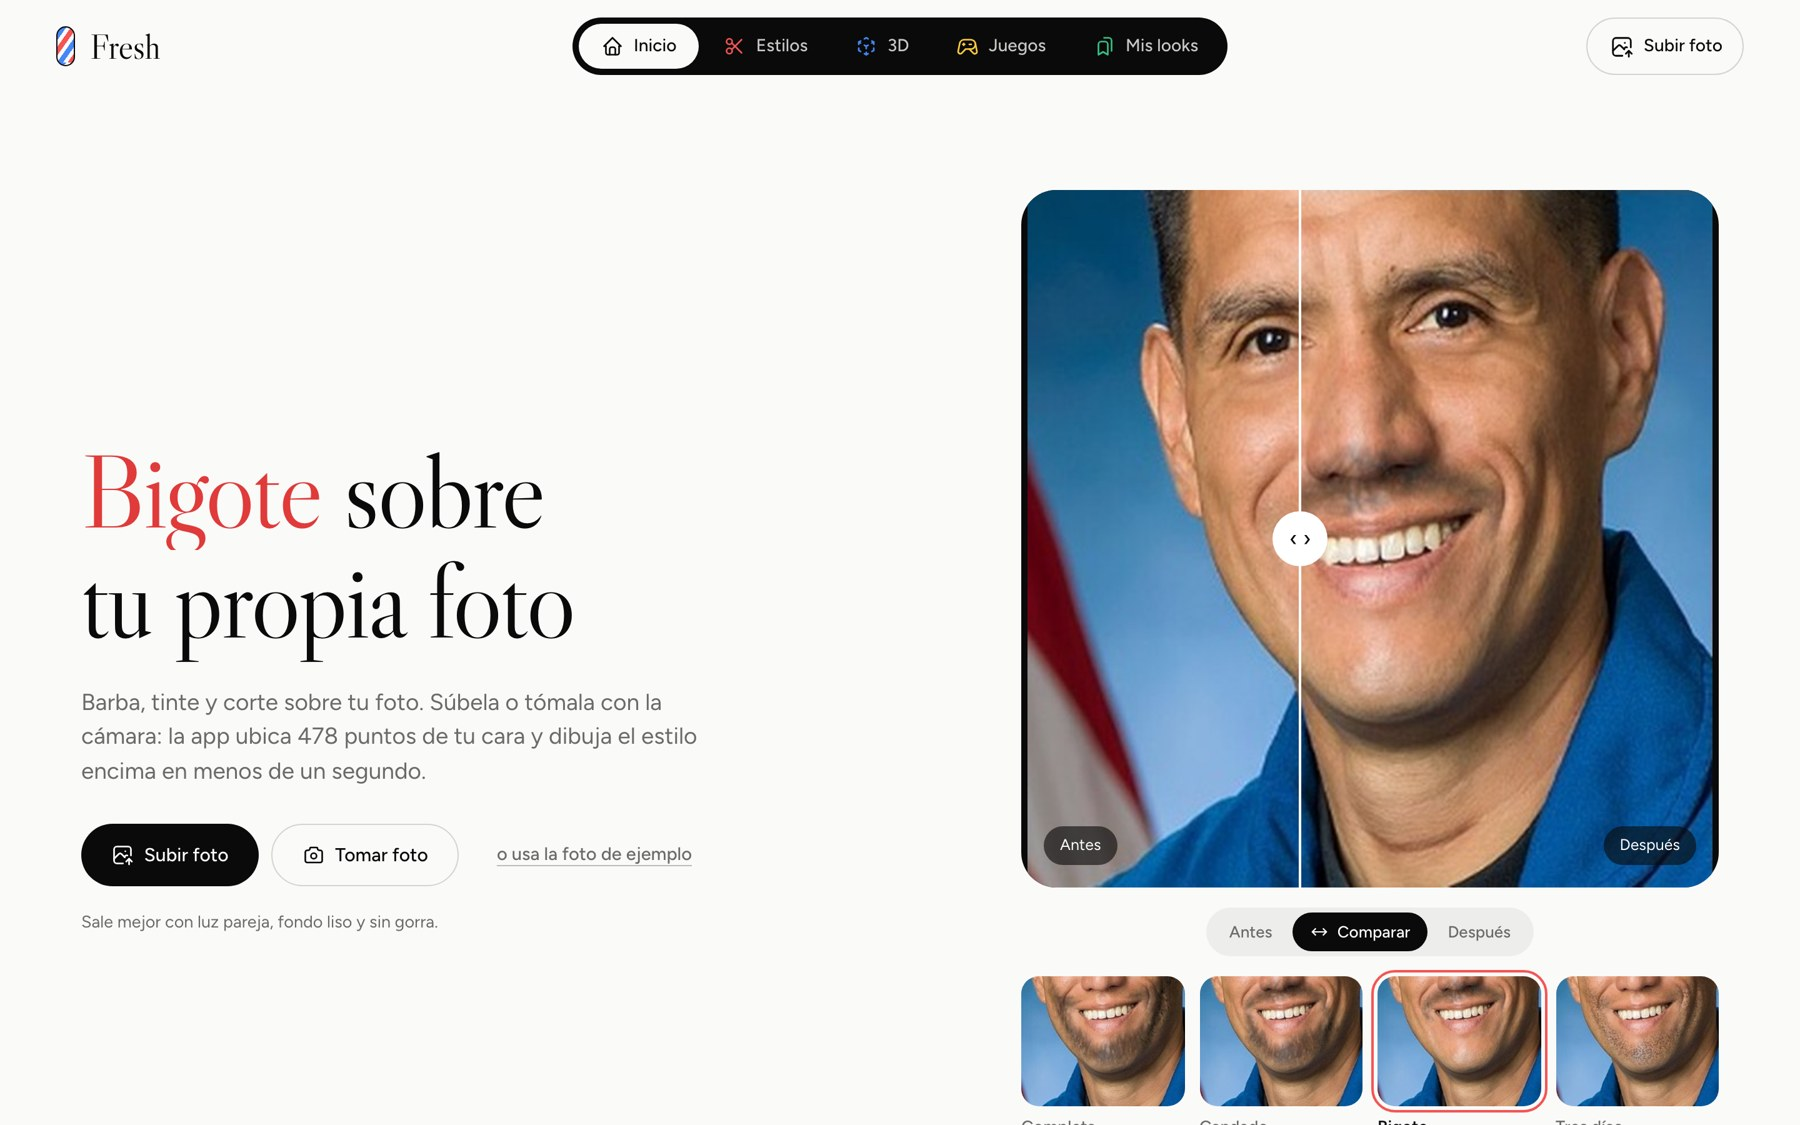
\includegraphics[width=0.92\linewidth]{ui_inicio.jpg}
  \caption{Pantalla de inicio de Fresh. La demostración de la derecha muestra un estilo de barba aplicado sobre un retrato de dominio público de la NASA.}
  \label{fig:inicio}
\end{figure}

\subsection{Relación con los temas del curso}
\label{sec:temas}

Los modelos preentrenados resuelven una sola pregunta: dónde están la cara, el pelo y la mano. Todo lo que la persona ve en pantalla lo calcula código del equipo. En el núcleo del servidor y el visor 3D hay unas 4\,000 líneas de algoritmos gráficos propios y unas 600 líneas que llaman a modelos, es decir, cerca del 87~\% es computación gráfica propia. La tabla~\ref{tab:temas} relaciona cada tema del sílabo del curso con la parte del proyecto que lo aplica.

\begin{table}[ht]
\centering
\small
\begin{tabularx}{\linewidth}{@{}>{\raggedright\arraybackslash}p{3.9cm} X l@{}}
\toprule
Tema del sílabo & Dónde se aplica en Fresh & Sección \\
\midrule
6.1.1 Teoría del color & Tinte en CIELAB; color de la barba en YCrCb; croma que baja en las sombras & \ref{sec:tinte}, \ref{sec:barba} \\
6.1.2 Representación de imágenes & Una foto como suma de gaussianas 2D; capas con alfa & \ref{sec:gauss2d} \\
6.1.3 Muestreo & Pirámide \emph{pull-push}; resolución de trabajo fija; gaussianas por área 3D con muestreo estratificado & \ref{sec:corte}, \ref{sec:espejo} \\
6.1.4 Interpolación & Bilineal propia en el \emph{warp}; baricéntricas para anclar hebras y gaussianas; curvas de Bézier y Chaikin & \ref{sec:barba}, \ref{sec:fisica} \\
6.2.1 Producto vectorial, áreas, Montecarlo & Orientación y área de triángulos; distancia punto--segmento del juego; inicialización aleatoria por importancia de las gaussianas 2D & \ref{sec:juego}, \ref{sec:gauss2d} \\
6.2.2 Línea de barrido y casco convexo & Fortune es un algoritmo de barrido; casco convexo para recortar regiones & \ref{sec:barba} \\
6.2.5 Voronoi y Delaunay & Cada evento de círculo de Fortune es un vértice de Voronoi y un triángulo de Delaunay & \ref{sec:barba} \\
6.3.1 GPU & \emph{Vertex} y \emph{fragment shaders} propios en WebGL2 & \ref{sec:espejo} \\
6.3.2 Procesamiento de mallas & Malla de 478 puntos elevada a 3D; normales y marcos tangentes; parametrización por triángulo con un marco local ortonormal & \ref{sec:espejo}, \ref{sec:lab} \\
6.3.3.1 Rasterización & El \emph{warp} recorre el rectángulo envolvente y prueba cada píxel con baricéntricas & \ref{sec:barba} \\
6.3.3.2 Iluminación y texturas & Lambert en el pelo corto; textura de barba por triángulo; textura de la peluca desde varias vistas & \ref{sec:corte}, \ref{sec:peluca} \\
6.3.3.3 Superficies visibles & Algoritmo del pintor: gaussianas ordenadas de atrás hacia adelante con \emph{counting sort} & \ref{sec:espejo} \\
6.3.3.5 \emph{Gaussian Splatting} & \emph{Render} 3DGS con proyección EWA y exportación \texttt{.ply}; gaussianas 2D ajustadas con gradientes analíticos & \ref{sec:espejo}, \ref{sec:gauss2d} \\
6.4.2 Bordes & Gradientes y tensor de estructura para la barba y la dirección del pelo & \ref{sec:barbatinte}, \ref{sec:peluca} \\
6.4.4 OpenCV & Lectura de imágenes, filtros, detector de Haar & \ref{sec:deteccion} \\
6.4.5--6.4.6 YOLO y ajuste fino & Segmentador de pelo entrenado por el equipo & \ref{sec:segmentacion} \\
\bottomrule
\end{tabularx}
\caption{Temas del sílabo de CS4016 que aplica el proyecto.}
\label{tab:temas}
\end{table}

Quedan fuera la transformada de Fourier (6.1.5), los \emph{kd-trees} (6.2.4), el \emph{windowing} (6.2.6), CUDA (6.3.1.2) y el trazado de rayos (6.3.3.3--6.3.3.4).

\subsection{Organización del documento}

La sección~\ref{sec:fundamentos} resume los fundamentos teóricos. La sección~\ref{sec:metodologia} describe los requisitos y la metodología de trabajo, y la sección~\ref{sec:arquitectura}, la arquitectura del sistema. La sección~\ref{sec:implementacion} detalla cada módulo con sus algoritmos, decisiones y limitaciones. La sección~\ref{sec:herramientas} indica qué herramienta resolvió cada parte, y la sección~\ref{sec:reproduccion} explica paso a paso cómo reproducir el proyecto. Los resultados se presentan en la sección~\ref{sec:resultados}, las limitaciones en la sección~\ref{sec:limitaciones} y las conclusiones en la sección~\ref{sec:conclusiones}.
